%% related-work.tex
%%

\chapter{Related Work}
\label{ch:related-work}

The ``Heisenberg Effect'' is described only in a few scientific papers. First mentioned in the paper by Bowman et al.~\cite{bowman_using_2001}, and picked up by Kopper et al~\cite{kopper_human_2010}, a real definition and evidence for the ``Heisenberg Effect'' were never given. In this section, a general definition, based on the previous works mentioned before, is drawn up and explained. To analyze and describe the Heisenberg Effect it is necessary to take a look at different researches on pointing tasks and the used procedures. Therefore, a detailed look at related work on 2D and 3D pointing tasks, spatial jitter, and resulting effects is given. Based on these papers this chapter is concluded by taking a look at underlying laws and algorithms which are used in the later study design to show and analyze the ``Heisenberg Effect''.

\section{Defining the Heisenberg Effect}
\label{sec:related-work:defining-heisenberg-effect}

\subsection{First reference by Bowman et al.}
\label{subsec:related-work:defining-heisenberg-effect:first-reference}

The first reference of the ``Heisenberg Effect'' was in the paper ``Using Pinch Gloves\textsuperscript{TM} for both Natural and Abstract Interaction Techniques in Virtual Environments'' by Bowman et al.~\cite{bowman_using_2001}. The paper shows the use of cloth gloves (called after the brand name ``Pinch Gloves\textsuperscript{TM}'') as input devices in virtual environments. They also describe different techniques to interact in VR with these gloves.  One problem they mentioned in their paper, was the difficulty to point at an object and simultaneously select it, without disturbing the previous pointing. This effect was called ``the Heisenberg Effect of spatial interaction''. To avoid this ``Heisenberg Effect'' while still using the selected gloves, they used one hand to point to the desired target and then the other hand to select it. More pieces of information or hints are not given by the mentioned paper. The meaning of the name ``Heisenberg Effect'' could be derived by ``Heisenberg's uncertainty principle'' in physics, declare it is only possible to either point on something with certainty or to select something with certainty. But not both at the same time.

\subsection{Description and link to Fitt's Law by Kopper et al.}
\label{subsec:related-work:defining-heisenberg-effect:description}

The term ``Heisenberg Effect'' was also used in the work of Kopper et al.~\cite{kopper_human_2010} called ``A human motor behavior model for distal pointing tasks''. This paper takes a focus on distal pointing tasks and gives an overview of different models to precisely measure movement time, by extending Fitt's Law. They conclude, that the natural hand jitter and the movement made while pressing down a button to select a target, add to an increase in movement time and difficulty. They call this effect also ``Heisenberg Effect'' and refer to the work of Bowman et al.~\cite{bowman_using_2001}.

\subsection{Own definition}
\label{subsec:related-work:defining-heisenberg-effect:definition}

Based on the previous work by Bowman and Kopper, the ``Heisenberg Effect'' in this thesis is defined as follows:

\begin{quote}
The ``Heisenberg Effect in distal pointing'' describes the difference between the position of a mental selection of a target and the real tracked position, distinguished by the disturbance of the selecting action.
\end{quote}

To show the ``Heisenberg Effect'' in an example, a look at Figure~\ref{fig:heisenberg_effect} shows a 
scenario, where a user is pointing with a controller via raycast on a target. The line P1 describes the acquired direction and aim of the user right before he is selecting the target by pressing or clicking a button. Trough the action of select the target, the raycast gets disturbed which is shown exemplarily by line P2. The now arising difference between ``wanted position'' and ``resulted position'' on the canvas is what was described previously and called the ``Heisenberg Effect'' (labeled as H1).

\begin{figure}[h]
    \centering
    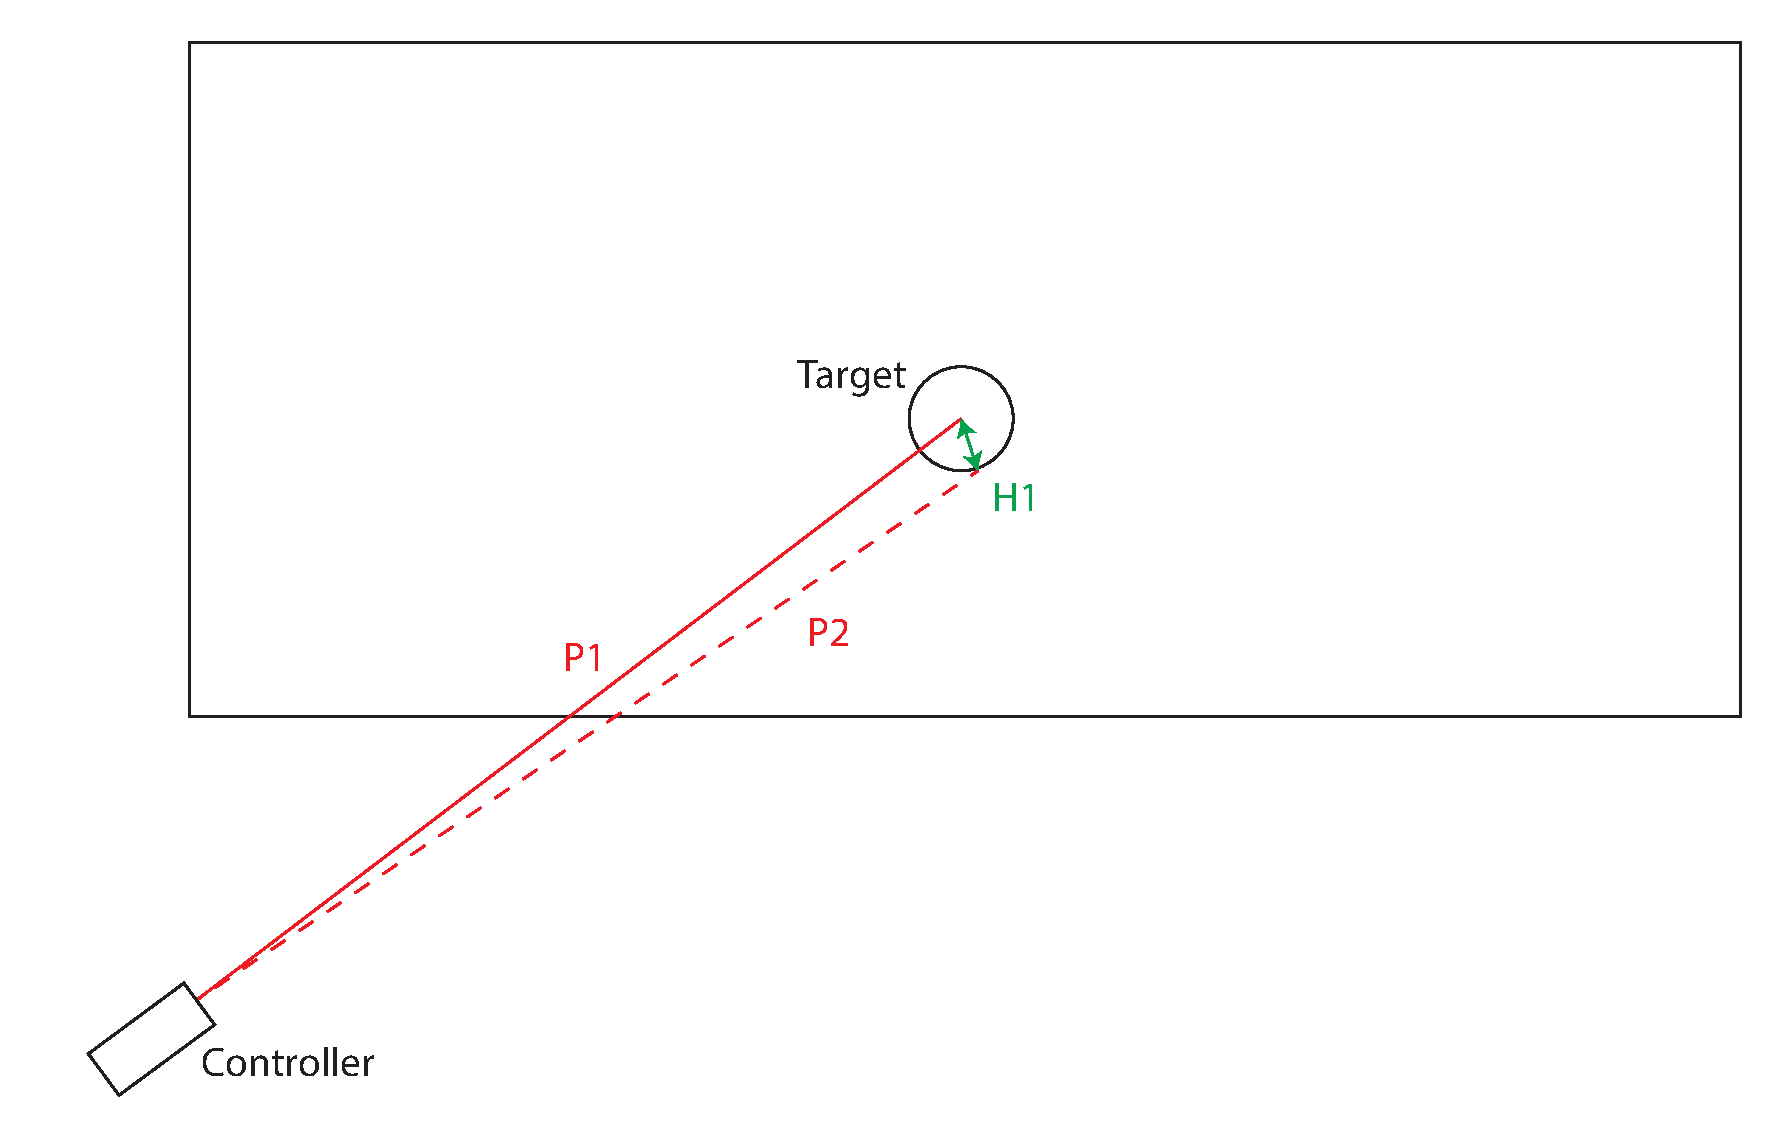
\includegraphics[width=.9\columnwidth]{graphics/heisenberg_effect.pdf}
    \caption{Describing the Heisenberg Effect on a simple distal pointing task example}
    \label{fig:heisenberg_effect}
\end{figure}

Based on this definition, this thesis wants to show, that the ``Heisenberg Effect'' exists, can be measured and therefore compensated.

\section{Background \& Related Work on pointing tasks}
\label{sec:related-work:pointion-tasks}

\subsection{Distal pointing tasks}

To measure and analyze accuracy in distal pointing, many studies use distal pointing tasks. In Figure~\ref{fig:pointing_task} a simple setup of such a task is shown. In VR the user handles with a controller a visible ray cast. This ray cast is a ray emitted from the tip of the controller in the given direction controlled by the user. If this ray cast hits a canvas the user can see, on which target on the canvas he points his controller (the ray cast is in Figure~\ref{fig:pointing_task} the red line P1). With a button on the controller, the user can select now a target on the canvas on which he is pointing at the moment he presses or clicks the button. In a distal pointing task, target after target is shown to the user and he has to move his controller in the direction of the target and select it with a press/click on the button.
These movements can be analyzed and described by Fitt's Law:

\subsection{Fitts' Law}
\label{subsec:related-work:background:fitts_law}

Fitts' Law is a model to calculate movement times and the difficulties of movements between a start point and a target or between two targets. The difficulty of such movements, called Index of Difficulty (\textit{ID}) and measured in bits, is described in one-dimension as:

\[\ ID = \log_2 (2 \cdot A / W) \]

where \textit{A} is the distance (or amplitude) between two targets and \textit{W} is the size of the target. In this work we use for \textit{ID} the so called ``Shannon formulation'' as suggested by MacKenzie and Buxton~\cite{mackenzie_extending_1992}, to scale on two-dimensions, fit better the observation and correct negative values for \textit{ID}:

\[ ID = \log_2 (A / W + 1) \]

\newpage

 Based on this Index of Difficulty, Fitts' Law describes the Movement Time (\textit{MT}) as follows:

\[ MT = a + b \cdot ID\]

a and b are empirically determined constant values based on the given input devices for the specific pointing task. Fitt's Law argues by these equations, that correct movements to targets get more difficult if the targets get smaller. With movement time (\textit{MT}) and \textit{ID}, we can calculate the throughput of an input device in bits per second:

\[ TP = ID / MT \]

\subsection{Extended Fitt's Law}
\label{subsec:related-work:background:extended_fitts_law}

In the study design for this work an extended model of the Fitt's Law, proposed by MacKenzie~\cite{mackenzie_fitts_law_reasearch_tool} and described on pointing tasks by Kong and Ren~\cite{kong_calculation_2006}, is used. MacKenzie claims in his paper, that the traditional Fitt's Law doesn't account the actual performance of a user when trying to hit small targets. For the extended
%Groß/Klein
Fitt's Law used here, the values for Distance and Width (now called \textit{Effective Distance} and \textit{Effective Width}) are calculated for the set of collected data. By using the standard deviation, the extended Fitt's Law can filter out different strategies used by the user to accomplish the tasks. MacKenzie described the \textit{Effective Witdh} as follows:

\[ W_e = 4.133 \cdot \sigma \]

where $\sigma$ is the standard deviation defined as:

\[ \sigma = \frac{\sum_{i=1}^{n} (x_i - \bar{x}) }{\sqrt{n - 1}}  \]

where $n$ is the number of trials and the sum describes the sum of deviations. As in the standard Fitt's Law the \textit{Effective Throughput} is defined here as:

\[ TP_e = \frac{ID_e}{MT_{mean}} \]

where 

\[ ID_e = \log_2 (\frac{A_e}{W_e} + 1) \]

\subsection{Related work on distal pointing}
\label{subsec:related-work:background:realted_work_on_distal_pointing}

The extended Fitt's Law is used in the work done by alternately Pavlovych, Stuerzlinger, MacKenzie and Teather~\cite{pavlovych_tradeoff_2009}~\cite{teather_effects_2009}~\cite{teather_pointing_2011} to analyze the effects of spatial jitter and lag on the performance in distal pointing tasks. Spatial jitter is described by Pavlovych and Stuerzlinger~\cite{pavlovych_tradeoff_2009} as ``a combination of hand tremor and noise in the device signal''. Their work gave a good foundation for the study design of this paper, mainly because of three reasons:

\begin{itemize}
    \item The study design in all three papers used the ISO 9241-9 specification~\cite{douglas_testing_1999} which gives clear conditions for this study design. Although the specification was not fully applied.
    \item To isolate the ``Heisenberg Effect'', it was important to clear our data from disturbances like the effects of hand tremor and noises of the device signals, described in their work.
    \item To give further works a base on how the ``Heisenberg Effect'' may affect performance in distal pointing tasks, by taking a look on the \textit{Effective Troughput} proposed by MacKenzie.
\end{itemize}




